\documentclass[a4paper]{report}
\usepackage{geometry}
\usepackage[pdftex]{color,graphicx}
\usepackage{listings}
\usepackage{hyperref}
\usepackage{float}
\usepackage{listings}
\usepackage{paralist}
\usepackage{pdfpages}
\usepackage{enumitem}
\usepackage{algorithmic}
\usepackage{algorithm}
\usepackage{longtable}
\usepackage{titlepic}
\usepackage{pdfpages}
\setcounter{tocdepth}{2}
\hypersetup{colorlinks,citecolor=black,filecolor=black,linkcolor=black,urlcolor=black}
\graphicspath{{UIScreenshots/}{ClassDiagrams/}}

\begin{document}
\chapter*{User Manual}
\label{sec:uman}
\subsection*{Installation}
\begin{enumerate}
\item Before the election a manager machine should be placed away from the voters and all the station machines should be placed so that they are accessible to the voters.
\item Install the ADO.NET 2.0 Provider for SQLite, (link \url{http://sourceforge.net/projects/sqlite-dotnet2/}) on each machine. This is the database framework needed to run the program.
\item Install Adobe acrobat reader, (link \url{http://get.adobe.com/reader/}) or another PDF reader on each machine. The user manual in the program is a PDF file and Adobe acrobat reader is able to display it.
\item Make sure that each machine is in the 192.168.0.1 - 192.168.255.255 IP range.
\item When using this application for the first time Windows will ask you if you want to allow Aegis DVL to pass through your firewall. You need to allow this.
\item Start the Digital Voter List application on each of the machines.
\item You are now presented with this screen: \\
\begin{center}
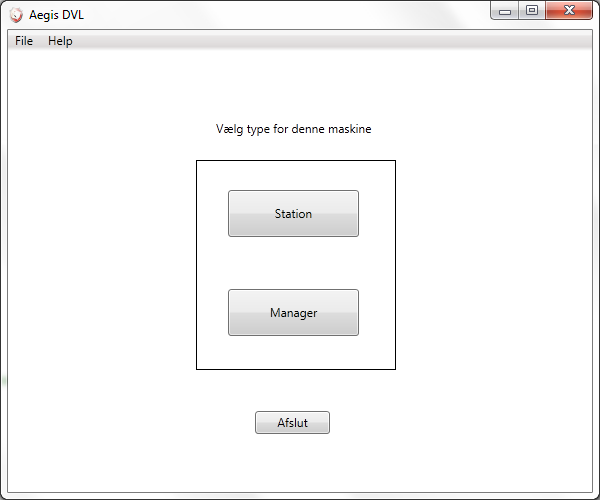
\includegraphics[width=100mm]{TypeChoice.png}
\end{center}
Choose Manager on the manager machine and Station on all the station machines.
\end{enumerate}

\subsection*{Station usage}
\begin{enumerate}
\item After you have selected Station you are presented with this page: \\
\begin{center}
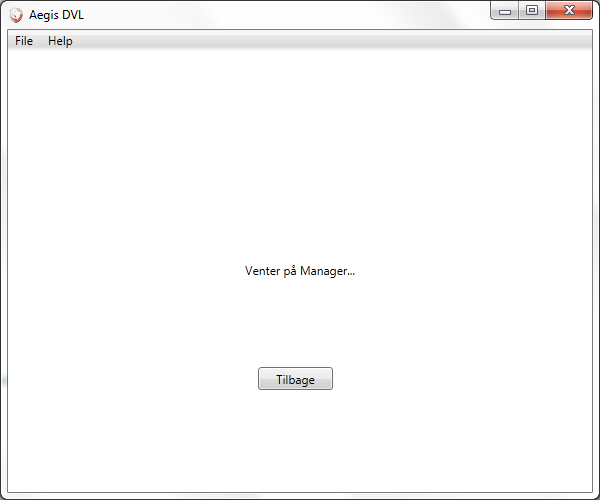
\includegraphics[width=100mm]{WaitingForManager.png}
\end{center}
This screen is displayed until a manager connects.
\item When a manager connects a password is shown on his screen and you are presented with this screen: \\
\begin{center}
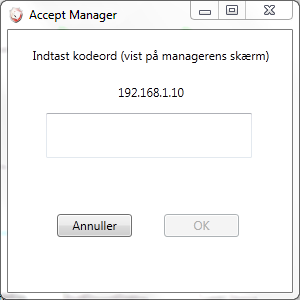
\includegraphics{AcceptManagerDialog.png}
\end{center}
Type the password displayed on the manager in this window and press OK.
\item When the password has been accepted, the reverse process begins. Now a password is displayed on your screen like this: \\
\begin{center}
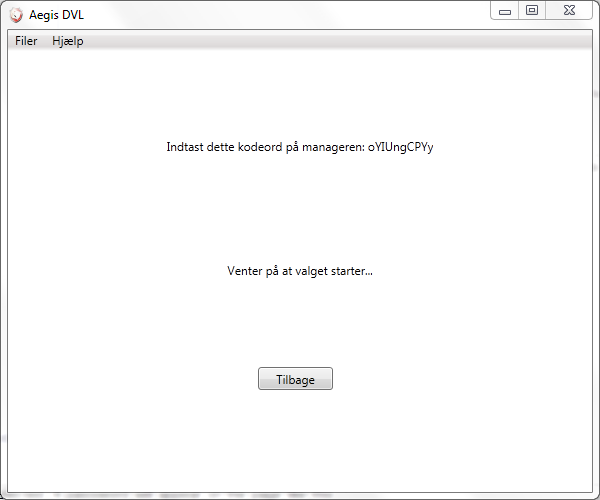
\includegraphics[width=100mm]{WaitingForManagerWithPassword.png}
\end{center}
Have the manager type this password in and the text on your screen switches to "Venter p\aa      \ at valget starter" which is displayed until the manager decides to start the election.
\item When the election starts you are presented with this screen: \\
\begin{center}
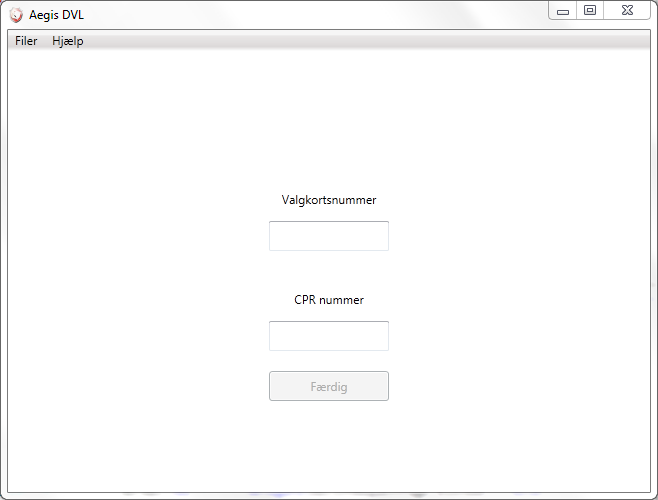
\includegraphics[width=100mm]{BallotRequest.png}
\end{center}
From this screen voters can scan/type their voter numbers and type in their CPR numbers. When this is done you can press "F\ae rdig" and one of the following dialogues is shown: \\
\begin{center}
 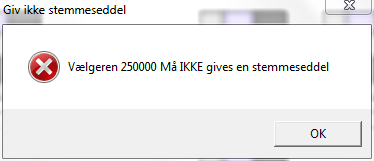
\includegraphics{BallotDenied.png}
\end{center}
This indicates that the voter is either not eligible to vote at this venue or that he has already been handed a ballot. \\
\begin{center}
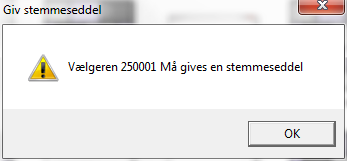
\includegraphics{BallotAccepted.png}
\end{center}
This indicates that the system has accepted the voter number and CPR number and that this voter can now be handed a ballot.
\item This process can be repeated until the manager decides that the election has ended.
\item When the election has ended the application automatically shuts down.
\item When the manager has exported the data and everyone is sure that the election has run as expected it is safe to delete the Voters.data file.
\end{enumerate}

\subsection*{Manager usage}
\begin{enumerate}
\item After you have selected Manager you are presented with this page: \\
\begin{center}
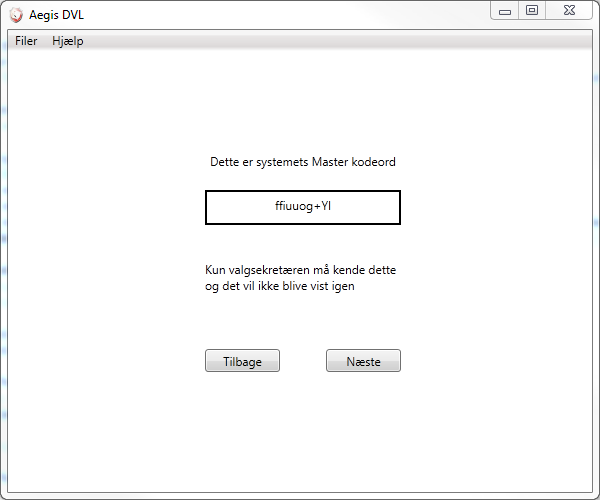
\includegraphics[width=100mm]{MasterPassword.png}
\end{center}
This window displays the master password. It should only be read by the election secretary and is never shown again! It is used to start an election, end an election, register a voter only with his CPR number and access the log database.
\item When you press "N\ae ste" you are presented with the Data Load Page: \\
\begin{center}
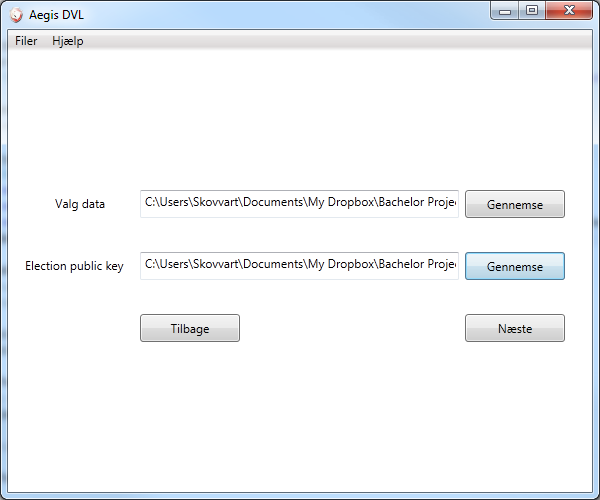
\includegraphics[width=100mm]{DataLoad.png}
\end{center}
From here you can choose the file location of the voter data the system needs to import and the encryption key for the voter data in question. When you have found these press "N\ae ste".
\item You are now presented with this page: \\
\begin{center}
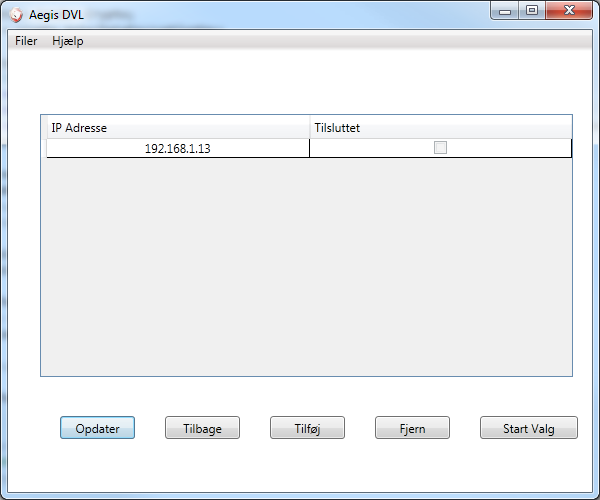
\includegraphics[width=100mm]{Overview.png}
\end{center}
From here you have several options. "Opdater" updates the list of stations you can connect to. "Tilbage" takes you back to the page showing the data loading. It generates a new master password which should be used henceforth. "Tilf\o j" attempts to connect to the station you have selected. A password appears on the page like this: \\
\begin{center}
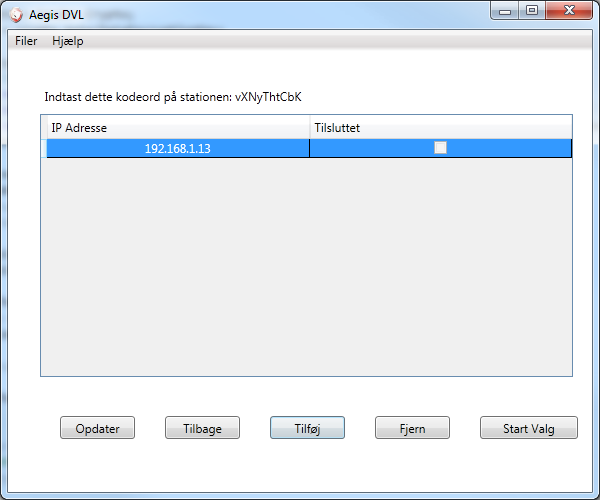
\includegraphics[width=100mm]{OverviewWithPassword.png}
\end{center}
and the station needs to input the password. After the station has entered the password and pressed "OK" you are asked for a password displayed on the station like this:
\begin{center}
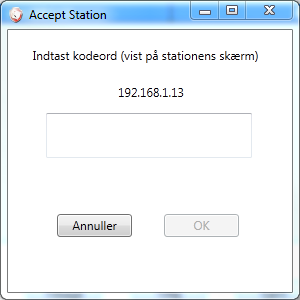
\includegraphics{AcceptStationDialog.png}
\end{center}
When you enter the right password the station appears as connected in the list. Pressing "Fjern" removes the stations as a peer, and announces to the remaining peers that they must do the same. A removed peer is ignored. "Start valg" asks you for the master password and start the election like so: \\
\begin{center}
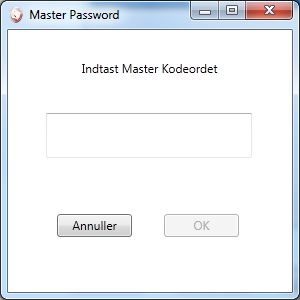
\includegraphics{CheckMasterPassword.png}
\end{center}
NOTICE: be aware that the system must always have at least four active machines to function. If this is not the case you are not able to start the election.
\item When the election has started you are presented with this page: \\
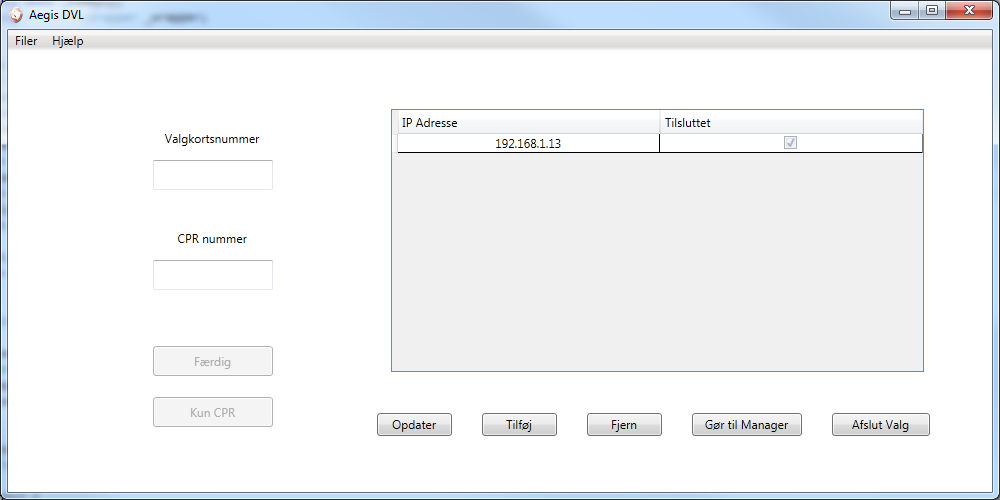
\includegraphics[width=\textwidth]{ManagerOverview.png}
This page is a combination of the previous page and the voting page from the station. The right side of the page functions exactly like the previous screen and the right side screen gives you the opportunity to mark voters with voter number and CPR number or just the CPR number provided you know the master password.
\item The only difference between the right side of the screen and the previous window is that the ''Start Valg'' have been replaced by ''Afslut Valg'' which lets you end the election provided you know the master password. When this is pressed the election ends, the station machines closes their applications and you are presented with this page: \\
\begin{center}
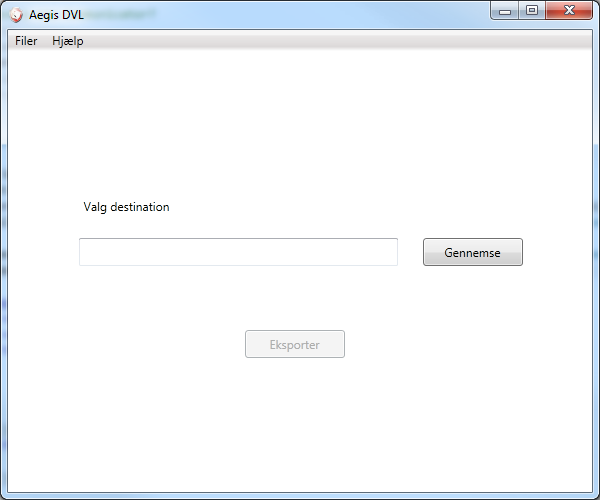
\includegraphics[width=100mm]{EndedElection.png}
\end{center}
\item Here you can export the voter data to a destination of your choice.
\end{enumerate}

\subsection*{Other}
At any time in the program you can choose "Marker v\ae lger", "Eksporter Data" or "Afslut" from the "Filer" menu or "Bruger manual" from the "Hj\ae lp" menu. \\
\begin{center}
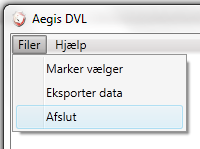
\includegraphics{FileMenu.png}
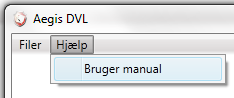
\includegraphics{HelpMenu.png}
\end{center}

\begin{itemize}
\item "Marker v\ae lger" opens this dialog: \\
\begin{center}
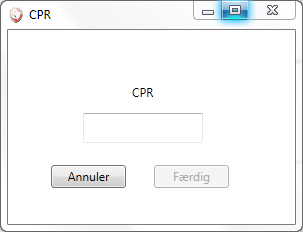
\includegraphics{BallotCPR.png}
\end{center}
Here you can mark a voter with only their CPR number, provided you know the master password. After you have entered the CPR number you are asked to enter the master password in this window: \\
\begin{center}
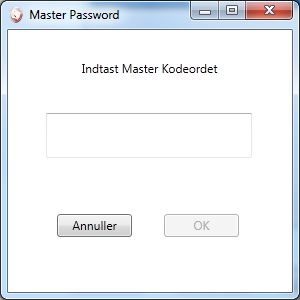
\includegraphics{CheckMasterPassword.png}
\end{center}
When this is done you can press ''OK'' and one of the following dialogues is shown: \\
\begin{center}
 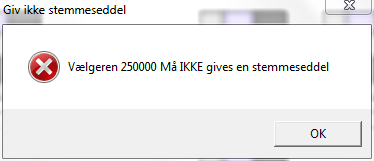
\includegraphics{BallotDenied.png}
\end{center}
This indicates that the voter is either not eligible to vote at this venue or that he has already been handed a ballot. \\
\begin{center}
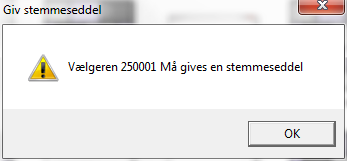
\includegraphics{BallotAccepted.png}
\end{center}
This indicates that the system has accepted the voter number and CPR number and that this voter can now be handed a ballot.

\item "Eksporter data" opens a dialog where you choose where to export the voter data. After you have chosen a destination, you are asked to enter the master password. When this is done successfully, the data is exported to the chosen location and the election continues.

\item ''Afslut'' asks you to enter the master password. If entered correctly, the application closes.

\item "Bruger manual" opens a PDF file containing this user manual.
\end{itemize}

If the manager machine should lose the connection to the network or lose power the remaining stations automatically elects one of the stations as the new manager and the user interface reflects it. \\

If the election should be a victim of an attack the detection triggers a shutdown of the entire election. This means this dialog appears on all machines: \\
\begin{center}
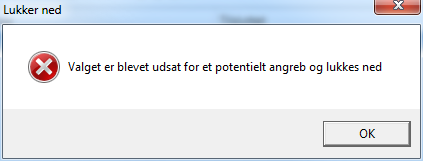
\includegraphics{ShutDownDialog.png}
\end{center}
When "OK" is pressed the application closes.

\end{document}